\documentclass[11pt]{article}
\usepackage{amsmath, amssymb, amsfonts}
\usepackage[margin=1in]{geometry}
\usepackage{fancyhdr}
\usepackage{tcolorbox}
\usepackage{enumerate}
\usepackage{tikz}
\usepackage{subcaption}

\usepackage{algorithmic}

\newcommand{\zo}{\{0,1\}}


\begin{document}

    \setlength{\headheight}{26pt}
    \pagestyle{fancy}
    \fancyhead[C]{\textbf{Basic Algorithms (Section 5)}\\Spring 2025}
    \fancyhead[R]{HW3 (Due 2/20 23:59)\\ Instructor: Jiaxin Guan}
    \fancyfoot[C]{}
    \fancyfoot[R]{\thepage}
    \renewcommand{\headrulewidth}{0.4pt}
    \renewcommand{\footrulewidth}{0.4 pt}
    
    %%%% EDIT THIS PART 
    %Put your name and Net ID here
    \fancyhead[L]{Name: Nick Zhu \\ Net ID: xz4687}
    %Write your collaborators' names here
    \fancyfoot[L]{Discussion Partners:}
    %%%%%
	
    
    %Problem 1
    \begin{tcolorbox}[title={Problem 1 (Divide and Conquer the Peak, 30 pts)}]
        Suppose we have an array $A$ of $n$ distinct integers and moreover are guaranteed that the array has the following property: up to some index $1\leq i \leq n$, $A$ is increasing, i.e., $A[1] < A[2] < \ldots < A[i]$, and then after index $i$, $A$ is decreasing, i.e., $A[i] > A[i+1] > \ldots > A[n]$. In this array, we call $A[i]$ the \emph{peak} of $A$. For example, consider the array $[1, 4, 7, 8, 6, 2]$, which has peak $8$. 
        \medskip
        
        Create an algorithm that finds the peak of an input array $A$ in sublinear time (i.e. $o(n)$). Justify the correctness and time complexity of your proposed algorithm.
    \end{tcolorbox}
    %Write your solution here!
    \section*{Solution}

    \textbf{Problem Statement:} \\
    Given an array \( A \) of \( n \) distinct integers that increases up to some index \( i \) (i.e., 
    \[
    A[1] < A[2] < \cdots < A[i]
    \]
    ) and then decreases (i.e., 
    \[
    A[i] > A[i+1] > \cdots > A[n]
    \]
    ), the element \( A[i] \) is the \emph{peak} of \( A \). For example, the array 
    \[
    [1,\, 4,\, 7,\, 8,\, 6,\, 2]
    \]
    has peak \( 8 \). Design an algorithm to find the peak in sublinear time (i.e., \( o(n) \)).
    
    \bigskip
    
    \textbf{Algorithm Description:} \\
    The key observation is that since the array is first increasing and then decreasing, a binary search can be employed to efficiently find the peak. Let \( \text{low} \) and \( \text{high} \) denote the current bounds of the search interval. At each step, compute
    \[
    \text{mid} = \left\lfloor \frac{\text{low} + \text{high}}{2} \right\rfloor.
    \]
    Then, compare \( A[\text{mid}] \) with \( A[\text{mid}+1] \):
    \begin{itemize}
        \item If \( A[\text{mid}] < A[\text{mid}+1] \), then the array is still increasing at \( \text{mid} \), so the peak must lie in the right half. Set \( \text{low} = \text{mid} + 1 \).
        \item Otherwise, if \( A[\text{mid}] > A[\text{mid}+1] \), then the peak is either at \( \text{mid} \) or to its left, so set \( \text{high} = \text{mid} \).
    \end{itemize}
    The loop terminates when \( \text{low} = \text{high} \), and at that point, \( A[\text{low}] \) is the peak.
    
    \bigskip
    
    \textbf{Pseudocode:}
    
    \begin{algorithmic}[1]
    \Procedure{FindPeak}{$A[1 \ldots n]$}
        \State \textbf{initialize} \( \text{low} \gets 1 \), \( \text{high} \gets n \)
        \While{\( \text{low} < \text{high} \)}
            \State \( \text{mid} \gets \left\lfloor \frac{\text{low} + \text{high}}{2} \right\rfloor \)
            \If{\( A[\text{mid}] < A[\text{mid}+1] \)}
                \State \( \text{low} \gets \text{mid} + 1 \)
            \Else
                \State \( \text{high} \gets \text{mid} \)
            \EndIf
        \EndWhile
        \State \textbf{return} \( A[\text{low}] \)
    \EndProcedure
    \end{algorithmic}[1]
    
    \bigskip
    
    \textbf{Correctness:} \\
    The algorithm maintains the invariant that the peak is always within the interval \([\,\text{low},\, \text{high}]\). At each iteration:
    \begin{itemize}
        \item If \( A[\text{mid}] < A[\text{mid}+1] \), the increasing property guarantees that the peak lies in the interval \([\text{mid}+1, \text{high}]\).
        \item If \( A[\text{mid}] \geq A[\text{mid}+1] \), the peak is in \([\text{low}, \text{mid}]\) since either \( A[\text{mid}] \) is the peak or the peak lies to its left.
    \end{itemize}
    When the loop terminates with \( \text{low} = \text{high} \), only one element remains, and by our invariant, it must be the peak.
    
    \bigskip
    
    \textbf{Time Complexity:} \\
    At each iteration, the search space is reduced by roughly half. Therefore, the number of iterations is \( O(\log n) \), which is sublinear with respect to \( n \).
    
    \bigskip
    
    \textbf{Conclusion:} \\
    The proposed binary search algorithm correctly identifies the peak element in a unimodal array in \( O(\log n) \) time.
x    
    
    \newpage
    
    %Problem 2
    \begin{tcolorbox}[title={Problem 2 (Two-Server Search, 35 pts)}]
        You have (limited) access to two databases, each of which contains $n$ numbers. For simplicity, you may assume each value across the $2n$ entries is unique. You may only query the databases in the following way: You give one of the databases an integer $1\leq k \leq n$, and it responds with the $k$-th smallest number in its database.
        \medskip
        
        Give a divide-and-conquer algorithm that finds the median value across all $2n$ entries using $O(\log n)$ queries to the servers. Justify the correctness and time complexity of your proposed algorithm.
    \end{tcolorbox}
    %Write your solution here!

    \newpage

    %Problem 3
    \begin{tcolorbox}[title={Problem 3 (Grid Tiling, 35 pts)}]
        For a positive integer $n$, consider a $2^n \times 2^n$ grid, where one of the unit squares is black and all others are white. Show that regardless of the position of the black unit square, the white area can be fully covered, without any overlapping, by L-shaped tiles consisting of $3$ unit squares (rotations are allowed).
        
        \bigskip
        
        {
        \centering
        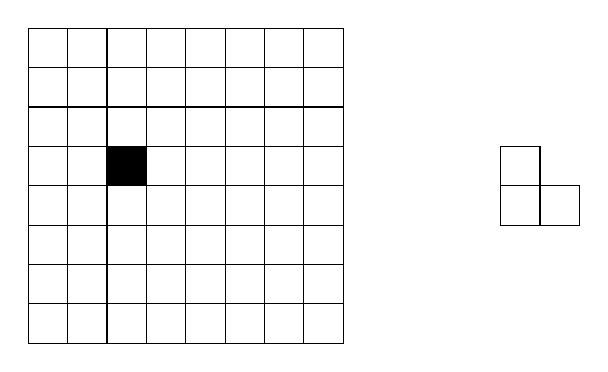
\begin{tikzpicture}[scale=0.5]
            \foreach \x in {0,1,...,7} {
                \foreach \y in {0,1,...,7} {
                    \fill[white,draw=black] (\x, \y) rectangle ++(1,1);
                }
            }
            % Fill one square with black
            \fill[black] (2, 4) rectangle ++(1,1);
            \fill[white,draw=black] (12, 3) rectangle ++(1,1);
            \fill[white,draw=black] (12, 4) rectangle ++(1,1);
            \fill[white,draw=black] (13, 3) rectangle ++(1,1);
        \end{tikzpicture}
        
        Left: an example grid with $n=3$; Right: the L-shaped tile
        
        }

        \bigskip
        
        (\emph{Hint: Use a proof by construction, i.e. design a divide-and-conquer algorithm that takes as input $n$ and $(i,j)$ with $1\leq i,j \leq 2^n$, and outputs a way to tile a $2^n\times 2^n$ grid with the black square at position $(i,j)$.}) 
        \medskip

             
    \end{tcolorbox}
    %Write your solution here!
    
    
\end{document}